% Instructions to change to html version:
% Comment out:
%  minipage, multicols,columnbreak, mathbf, hrule
% Replace all: \begin{minipage}% \end{minipage} %\begin{multicols}  %\end{multicols}  %\columnbreak %% \begin{framed} %\end{framed} %%\hrule
% Replace \mathbf with \boldsymbol
% Replace $$ with \[ or \]and $ with \( or \)
% Enclose graphics in figure environments and add captions
% 			search \includegraphics
% Re-tag \df environments as sections, subsections, etc.
% Command Line Code to Create html version:
%First: pdflatex -shell-escape filename.tex                                   
%Second, for each figure: inkscape "filename-figure1.pdf" -o "filename-figure1.png"
% Third: htlatex filename.tex "ht5mjlatex.cfg, charset=utf-8" " -cunihtf -utf8"

\documentclass[10pt]{article}

%\usepackage{tikz, pgf,pgfplots,wasysym,array}
%\usepackage{wasysym,array}

\usepackage{amsmath,amssymb}

\ifdefined\HCode
  \def\pgfsysdriver{pgfsys-tex4ht-updated.def}
\fi 
%\ifdefined\HCode
%  \def\pgfsysdriver{pgfsys-dvisvgm4ht.def}
%\fi 
\usepackage{tikz}
\usetikzlibrary{calc,decorations.markings,arrows}
\usepackage{pgfplots}

\pgfplotsset{compat=1.12}
\usepackage{myexternalize}
\usetikzlibrary{calc,decorations.markings,arrows}
\usepackage{framed}
\usepackage[none]{hyphenat}

\input{../../../common/1336_header_test.tex}
\begin{document}

\everymath{\displaystyle}


\newcommand{\ihat}{\boldsymbol{\hat{\textbf{\i}}}}
\newcommand{\jhat}{\boldsymbol{\hat{\textbf{\j}}}}
\newcommand{\khat}{\boldsymbol{\hat{\textbf{k}}}}

\let\oldvec\vec
\renewcommand{\vec}[1]{\oldvec{\boldsymbol{#1}}}

\renewcommand{\u}{\vec{u}}
\renewcommand{\v}{\vec{v}}
\newcommand{\w}{\vec{w}}
\renewcommand{\r}{\vec{r}}
\renewcommand{\a}{\vec{a}}
\renewcommand{\b}{\vec{b}}

\newcommand{\<}{\langle}
\renewcommand{\>}{\rangle}

\renewcommand{\myTitle}{MATH 1336: Calculus III}

\renewcommand{\mySubTitle}{Section 2.5, Part 1: Lines \vspace*{-.2in}}
%~\hfill Name: \underline{~~~~~~~~~~~~~~~~~~~~~~~~~~~~~~~~~~~~~~~~~~~~~~~}

\lectTitle{\vspace*{-.5in}\myTitle}{\vspace*{.1in}\mySubTitle \vspace*{-.1in}}


\setlength{\columnseprule}{0.4pt}
\setlength{\columnsep}{3em}

%\hspace*{-.8in}%\begin{minipage}{1.25\textwidth}
%\begin{framed}


\section*{Equations of Lines: }

In \(\mathbb{R}^2\) (the coordinate plane), we know that a point and a slope can be used to determine an equation for a line, using the point-slope formula:

\[ y - y_1 = m (x - x_1)\]




We build on that idea to determine equations of lines in in \(\mathbb{R}^3\): a point, \(P_0 = (x_0, y_0, z_0)\) and a direction, \(\v = \<a, b, c\>\), can be used to determine an equation of a line.\\

Let \(\vec{r}_0 = \<x_0, y_0, z_0\>\) be the position vector for the point \(P_0\), \(\vec{r}  = \< x, y, z\>\) be the position vector for any general point \(P = ( x, y, z)\) on the line \(L\), and let \(\v = \<a, b, c\>\) be any vector parallel to the line.\\
  Then the line can be described by any of the following types of equations:\\

%\begin{minipage}{.4\textwidth}


\begin{figure}[!h]
\centering
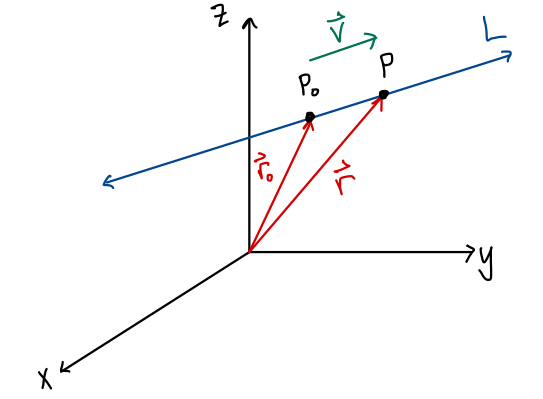
\includegraphics[width=\textwidth]{Ch10s5-lines2.png}
\caption{Diagram illustrating equations of lines in three dimensions.}
\end{figure}



%\end{minipage}
\hspace*{.2in}
%\begin{minipage}{.5\textwidth}





\textbf{Vector Equation:}

\[
\r = \r_0 + t \v
\]
~\\

\textbf{Parametric Equations:}

\[
x = x_0 + a t, \qquad y = y_0 + b t, \qquad z = z_0 + c t
\]

~\\

\textbf{Symmetric Equations:}\\

\[
\frac{x-x_0}{a} = \frac{ y - y_0}{b} = \frac{z - z_0}{c}
\]

~\\

%\end{minipage}

Note that \(a, b, c\) are sometimes called the \textbf{direction numbers} of the line.

%\end{framed}
%\end{minipage}


%
%\begin{framed}
%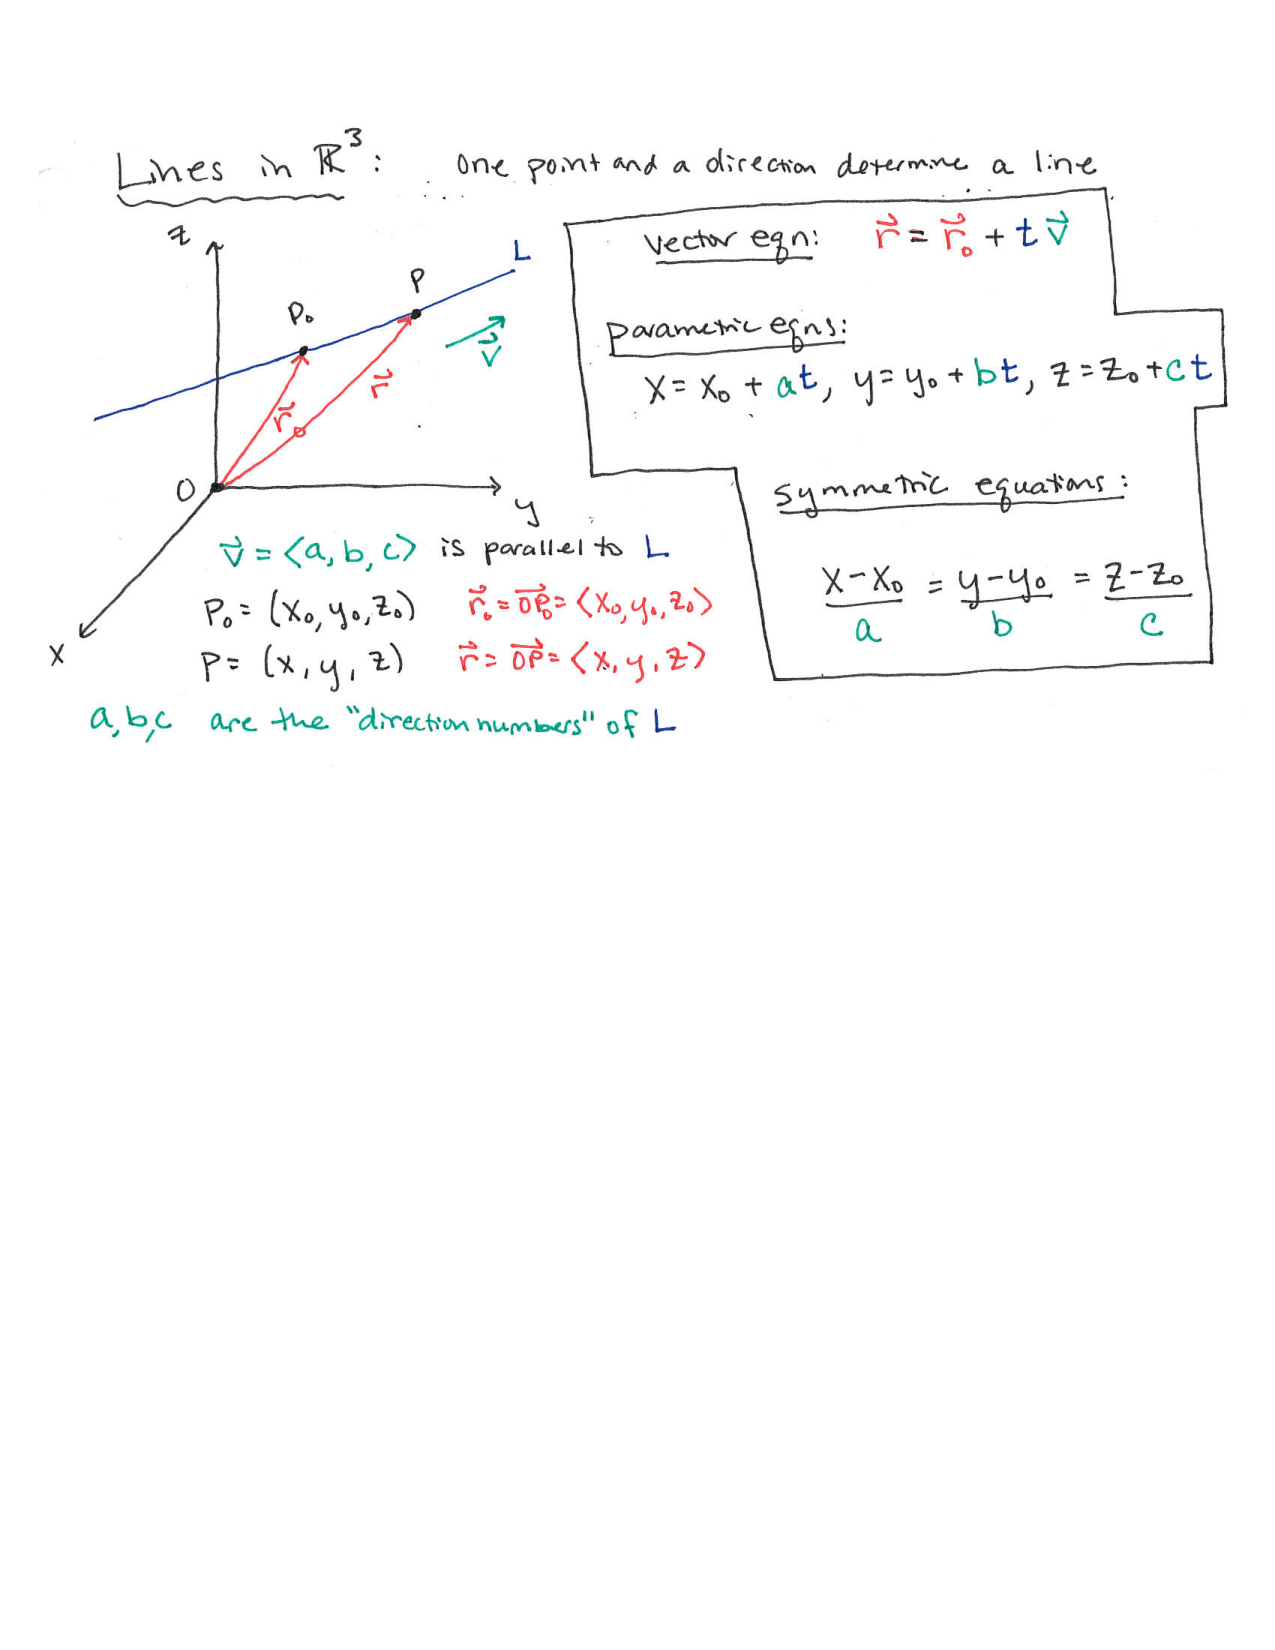
\includegraphics[width=\textwidth]{Ch10s5-lines.pdf}
%\end{framed}

\section*{Example 1:}% (Pre-class Video):} 

%\newcounter{prob}
%
%\begin{list}{\bf{Example \arabic {prob}: }}{\usecounter{prob}}
%\item \textbf{(Pre-Class Video Solutions)}\\
Find vector, parametric, and symmetric equations for the line that passes through the points\\ \(
A = (0,0,4),\) and \( B = (12, 8, 8).\)\\
%\[
%A = (0,0,4), \quad \text{and} \quad B = (12, 8, 8)
%\]
\hrule

In order to build our line equations, we need to find an initial vector \(\r_0\), and a vector \(\v\) parallel the the line.\\
 We can pick \textit{either} one of the given points for \(\r_0\), so I decided to choose \(\r_0 = \<0, 0, 4\>\).

To find \(\v\), we can calculate the vector that points from \(A\) to \(B\):
\[
\v = \overrightarrow{AB} = \<12-0, 8-0, 8-4\> = \<12, 8, 4\>
\]

%We can use these two vectors to build the requested different types of line equations:


\textbf{Vector Equation:}
\(\quad
\r = \r_0 + t \v = \<0, 0, 4\> + t \<12, 8, 4\> = \<12t, 8t, 4+4t\>
\)


\textbf{Parametric Equations:}
\(\quad
x = 12 t, \qquad y = 8 t, \qquad z = 4 + 4 t
\)



\textbf{Symmetric Equations:}
\(\quad
\frac{x}{12} = \frac{ y }{8} = \frac{z - 4}{4}
\)




\pagebreak

\section*{Example 2:} 
%\item
Show that the lines below are \textbf{skew lines}: they are not parallel and do not intersect one another.

\[
L_1: \qquad x -1 = \frac{y+2}{3} = 4-z, \qquad \qquad 
L_2: \qquad \frac{x}{2} = y-3 = \frac{z+3}{4}
\]

%\end{list}
%\pagebreak
\vfill
\vfill

\section*{Lines Practice Problems:}

\newcounter{prob}

\begin{list}{\bf{Problem \arabic {prob}: }}{\usecounter{prob}}

\item Find parametric equations for the line that passes through \(P=(3,1,4)\) and is parallel to the vector \(\v = -\ihat + \jhat -2\khat\).  Then find the points where the line passes through the coordinate planes and use the information to sketch the line.% in the space below.

\vfill

\item Find the vector equation for the line that passes through the points \((-1, 3, 7)\) and \((4, 2, -1)\).

\vfill

\item  Show that the lines
\[
L_3:\qquad \frac{x-1}{2}= \frac{y+1}{1} = \frac{z-2}{4}, \qquad\qquad L_4: \qquad \frac{x+2}{4} = \frac{y}{-3} = \frac{z-\tfrac{1}{2}}{-1}
\]
intersect, and find the point of intersection.

\vfill

\end{list}

\end{document}
